%%%%%%%%%%%%%%%%%%%%%%%%%%%%%%%%%%%%%%%%%%%%%%%%%%%%%%%%%%%%%%%%%%%%%%%%

\frame{
\frametitle{Outline}
\begin{itemize}
  \item Why Bayesian methods? 
  \vspace{2mm}
  \item Likelihood, prior and posterior: how are they connected?
  \vspace{2mm}
  \item Bayes's theorem and example in diagnostic setting
  \vspace{2mm}
  \item  Inference on proportions: Binomial-Beta models
  \vspace{2mm}
   \item \alert{Inference on continuous data: Normal-Normal models}
   \vspace{2mm}
  \item \alert{Inference on count data: Poisson-Gamma models}

\end{itemize}
}

%%%%%%%%%%%%%%%%%%%%%%%%%%%%%%%%%%%%%%%%%%%%%%%%%%%%%%%%%%%%%%%%%%%%%%%%
\section{Inference on continuous data: Normal-Normal models}
\frame{\frametitle{Conjugate Bayesian inference for continuous data: THM example}
\begin{itemize}
\item Regional water companies in the UK are required to take routine measurements
   of trihalomethane (THM) concentrations in tap water samples for regulatory purposes
\item Samples are tested throughout the year in each water supply zone
\item Suppose we want to estimate the mean THM concentration
    in a particular water zone
\item Two independent measurements, $y_{1}$ = 128$\frac{\mu g}{l}$ and $y_{2}$=132$\frac{\mu g}{l}$ are taken,
   and their mean, $\overline{y}$, is 130$\frac{\mu g}{l}$
\item Suppose we know that the true standard deviation of THM measurements in this water zone is
   $\sigma= 5\frac{\mu g}{l}$ (from the known assay measurement error)
\item What should we estimate the mean THM concentration to be in this water zone?
\end{itemize}

 Denote the mean THM concentration for the zone by $\theta$

}
%%%%%%%%%%%%%%%%%%%%%%%%%%%%%%%%%%%%%%%%%%%%%%%%%%%%%%%%%%%%%%%%%%%%%%%%
\frame{
\frametitle{Frequentist analysis}

 \bibig
 \I A standard analysis
would use the sample mean $\overline{y}$ = 130$\frac{\mu g}{l}$ as an estimate of $\theta$,
with standard error $\frac{\sigma}{\sqrt{n}} =\frac{5}{\sqrt{2}} = 3.5\frac{\mu g}{l}$ \vspace{2mm}

\I A 95\% confidence interval is $\overline{y} \pm 1.96 \times
\frac{\sigma}{\sqrt{n}}$, i.e.~123.1 to 136.9 $\frac{\mu g}{l}$
\eibig

}
%%%%%%%%%%%%%%%%%%%%%%%%%%%%%%%%%%%%%%%%%%%%%%%%%%%%%%%%%%%%%%%%%%%%%%%%
%%%%%%%%%%%%%%%%%%%%%%%%%%%%%%%%%%%%%%%%%%%%%%%%%%%%%%%%%%%%%%%%%%%%%%%%
\frame{
\frametitle{Bayesian analysis}


As we did previously with the Binomial-Beta model, try to think of the two components which we need to perform Bayesian inference:\vspace{2mm}

\begin{itemize}
  \item Likelihood (distribution of the data)\vspace{2mm}
  \item Prior belief\vspace{2mm}
\end{itemize}


}



\begin{frame}[containsverbatim]

\frametitle{Components of a Bayesian analysis}

\textbf{Likelihood}:

\begin{center}\vspace{-1mm}$y_i \sim {\rm N}(\theta,
\sigma^2) \hspace{10pt} (i=1,...,n)$\end{center}\vspace{-1mm}

N.B. Here we assume that $\sigma^2$ is known

\vspace{10pt}

\textbf{$\theta$ is given a prior distribution}:

\begin{center}\vspace{-1mm}
$\theta \sim {\rm N}(\mu, \omega^2)$
\end{center}\vspace{-2mm}
\bi
\I It is convenient to write the prior variance as a function of the data variance, i.e.~$\omega^2 = \frac{\sigma^2}{n_0}$\vspace{2mm}
\I We will see that $n_0$ ($=\frac{\sigma^2}{\omega^2}$) can be interpreted as an implicit prior sample size\vspace{2mm}
\ei

OpenBUGS notation: \verb" y ~ dnorm(theta, tau)" where {\tt tau} is the inverse of the variance
\end{frame}

%%%%%%%%%%%%%%%%%%%%%%%%%%%%%%%%%%%%%%%%%%%%%%%%%%%%%%%%%%%%%%%%%%%%%%%%%%%%
\frame{

\frametitle{Specifying values for the parameters of the prior}
\bibig
\I Suppose historical data on THM levels in other zones supplied from the same source
showed that the average of the zone-specific mean THM concentrations was 120 $\frac{\mu g}{l}$ with standard deviation
10 $\frac{\mu g}{l}$\vspace{2mm}
\item Suggests ${\rm N}(120, 10^2)$ prior for  $\theta$\vspace{2mm}
 \item Expressing the prior standard deviation as a function of the sampling standard deviation, $\omega^2 = \frac{\sigma^2}{n_0}$, and solving for $n_0$ gives $n_0 = \frac{\sigma^2}{\omega^2} = \frac{5^2}{10^2} = 0.25$\vspace{2mm}
\item So our prior can be written as $\theta \sim {\rm N}(120, \frac{\sigma^2}{0.25})$\vspace{2mm}
\item As $n_0$ tends to 0, the prior variance becomes larger and the distribution becomes `flatter'
\ei
}
%%%%%%%%%%%%%%%%%%%%%%%%%%%%%%%%%%%%%%%%%%%%%%%%%%%%%%%%%%%%%%%%%%%%%%%%%%%%
%http://www2.bcs.rochester.edu/sites/jacobslab/cheat_sheet/bayes_Normal_Normal.pdf

\frame{
	\frametitle{Combining prior and likelihood}
	
	Combining the Normal likelihood and the Normal prior

\alert{	
	\begin{equation*}
		p(\mathbf{y}|\theta) = \prod_{i=1}^n \frac{1}{{\sigma \sqrt {2\pi } }}e^{{{ - \left( {y_i - \theta } \right)^2 } \mathord{\left/ {\vphantom {{ - \left( {y_i - \theta } \right)^2 } {2\sigma ^2 }}} \right. \kern-\nulldelimiterspace} {2\sigma ^2 }}}
	\end{equation*}
	
	\begin{equation*}
		p(\theta) = \frac{1}{{ \sqrt {2\pi (\sigma^2/n_0)} }}e^{{{ - \left( {\theta - \mu } \right)^2 } \mathord{\left/ {\vphantom {{ - \left( {\theta - \mu } \right)^2 } {2 (\sigma^2/n_0) }}} \right. \kern-\nulldelimiterspace} {2 (\sigma^2/n_0) }}}
	\end{equation*}
	
	\begin{equation*}
	p(\theta|\mathbf{y})\propto \frac{1}{{\sqrt {\sigma^{2n} (\sigma^2/n_0)} }} e^{\frac{-\left( {\theta - \mu } \right)^2 }{2 (\sigma^2/n_0) } + \frac{-\sum_{i=1}^n \left( y_i - \theta \right)^2 }{2 \sigma^2 }}
	\end{equation*}}

After some algebra the exponent can be rearranged to
\alert{
	\begin{equation*}
		- \frac{1}{2}\left[ \frac{ \left(\theta - \frac{n_0\mu + n\overline{y}}{n_0 + n} \right)^2}{\frac{\sigma^2}{n_0 +
				n}} \right]
	\end{equation*}
}}



\frame{
\frametitle{Combining prior and likelihood}

Combining the Normal likelihood and the Normal prior gives the following posterior distribution
\alert{\begin{eqnarray*}
\theta\mid \mathbf{y} &\sim& {\rm N}\left(
\frac{n_0\mu + n\overline{y}}{n_0 + n} , \frac{\sigma^2}{n_0 +
n}\right)\\[3pt]
& \sim& {\rm N}\left(
\frac{0.25\times 120 + 2\times 130}{0.25 + 2} , \frac{5^2}{0.25 +
2}\right)\\[3pt]
&=& {\rm N}(128.9, \hspace{10pt} 3.33^2)
\end{eqnarray*}
}
This gives 95\% posterior interval for $\theta$ of  122.4 -- 135.4 $\frac{\mu g}{l}$

\small
\begin{itemize}
\item Posterior mean
 $\frac{(n_0\mu + n\overline{y})}{(n_0 + n)}$ is a weighted average of
 the prior mean $\mu$ and parameter estimate $\overline{y}$, weighted by their
 precisions (relative `sample sizes') $\rightsquigarrow$ compromise between the two\vspace{1mm}
\item Posterior variance is based on an implicit sample
   size equivalent to the sum of the prior `sample size'
   $n_0$ and the sample size of the data $n$ \vspace{1mm}
\item As $n\rightarrow \infty$,  $p(\theta \mid  \mathbf{y}) \rightarrow
\hbox{N}(\overline{y},\frac{\sigma^2}{n}) $ which does not depend on the
prior
%\item Compare with frequentist setting, the MLE is $\hat{\theta}=\bar{y}$ with
%SE$(\hat{\theta})=\sigma/\sqrt{n}$, and sampling distribution
%$
%p(\hat{\theta} \mid \theta) = p(\bar{y}\mid \theta) =
%\mathrm{N}(\theta,\, \sigma^2/n)
%$
\end{itemize}
\normalsize
}

\frame{

 \frametitle{Prior, likelihood and posterior for THM example}


\vspace{-35pt}
\centerline{\scalebox{0.8}{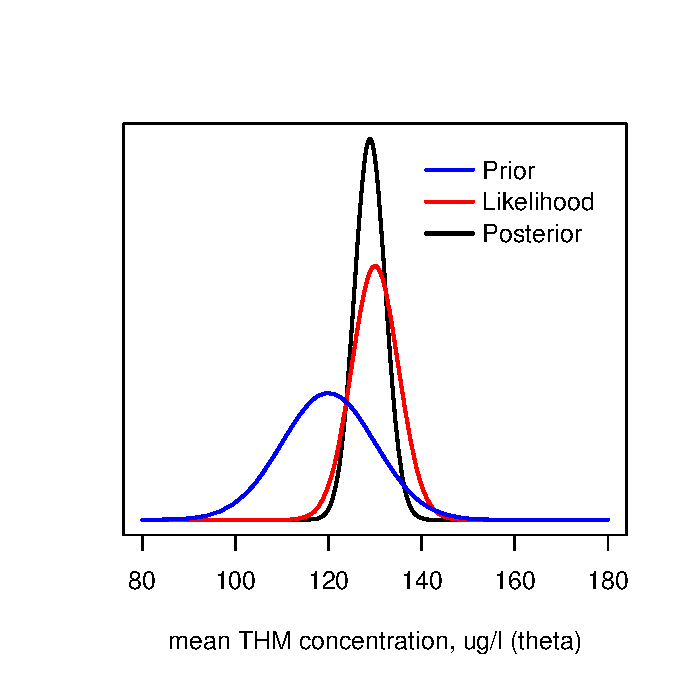
\includegraphics{Figures/thm-prior-like-post.pdf}}}
\begin{center}
\end{center}
}
%%%%%%%%%%%%%%%%%%%%%%%%%%%%%%%%%%%%%%%%%%%%%%%%%%%%%%%%%%%%%%%%%%%%%%%%
\section{Inference on count data: Poisson-Gamma models}
\frame{
\frametitle{Bayesian inference using count data}

Suppose we have an independent sample of counts $y_1,\ldots,y_n$ which
can be assumed to follow a Poisson distribution with unknown mean
$\mu$:

\alert{\begin{equation*}
p(\mathbf{y}\mid \mu) = \prod_i \frac{\mu^{y_i}e^{-\mu} }{y_i!}
\end{equation*}
}
 The conjugate prior for the mean of a Poisson distribution is a
Gamma distribution:
\alert{\begin{equation*}
p(\mu) = \hbox{Gamma}(a, b) = \frac{b^a}{\Gamma(a)} \mu^{a-1} e^{-b
\mu}
\end{equation*}
}
}
%%%%%%%%%%%%%%%%%%%%%%%%%%%%%%%%%%%%%%%%%%%%%%%%%%%%%%%%%%%%%%%%%%%%%%%%

\begin{frame}[containsverbatim]
\frametitle{The Gamma distribution}

Flexible distribution for positive quantities \vspace{2mm}

If $\mu \sim {\rm Gamma}[a,b]$
  \begin{eqnarray*}
p(\mu \mid a, b) & = & \frac{ b^a }{\Gamma(a) } \mu^{a-1} \ e^{-b\mu}, \hspace{10pt} \mu \in (0,\infty)   \\[5pt]
{\rm E}(\mu  \mid a, b) &= &   \frac{a}{ b }     \\[5pt]
{\rm V}(\mu  \mid a, b) &= &   \frac{a}{ b^2 }
\end{eqnarray*}

OpenBUGS notation:  \verb"mu ~ dgamma(a,b)"
\end{frame}

\begin{frame}[containsverbatim]
\frametitle{The Gamma distribution [continued]}
\begin{itemize}
\item  Gamma[1,$b$] distribution is exponential with mean $\frac{1}{b}$\vspace{2mm}
\item  Gamma[$\frac{v}{2},\frac{1}{2}$] is a Chi-squared $\chi^2_v$ distribution on $v$ degrees of freedom\vspace{2mm}
\item $\mu \sim $ Gamma[0,0] means that $p(\mu) \propto \frac{1}{\mu}$, or that $\log \mu \sim$ Uniform\vspace{2mm}
\item Also used as conjugate prior distribution for inverse variances (precisions) of Normal distributions\vspace{2mm}
\item Can also be used as sampling distribution for skewed positive valued quantities (alternative to log normal likelihood)
\end{itemize}
\end{frame}

\begin{frame}
    \frametitle{Shape of the Gamma distribution}
    \scalebox{0.6}{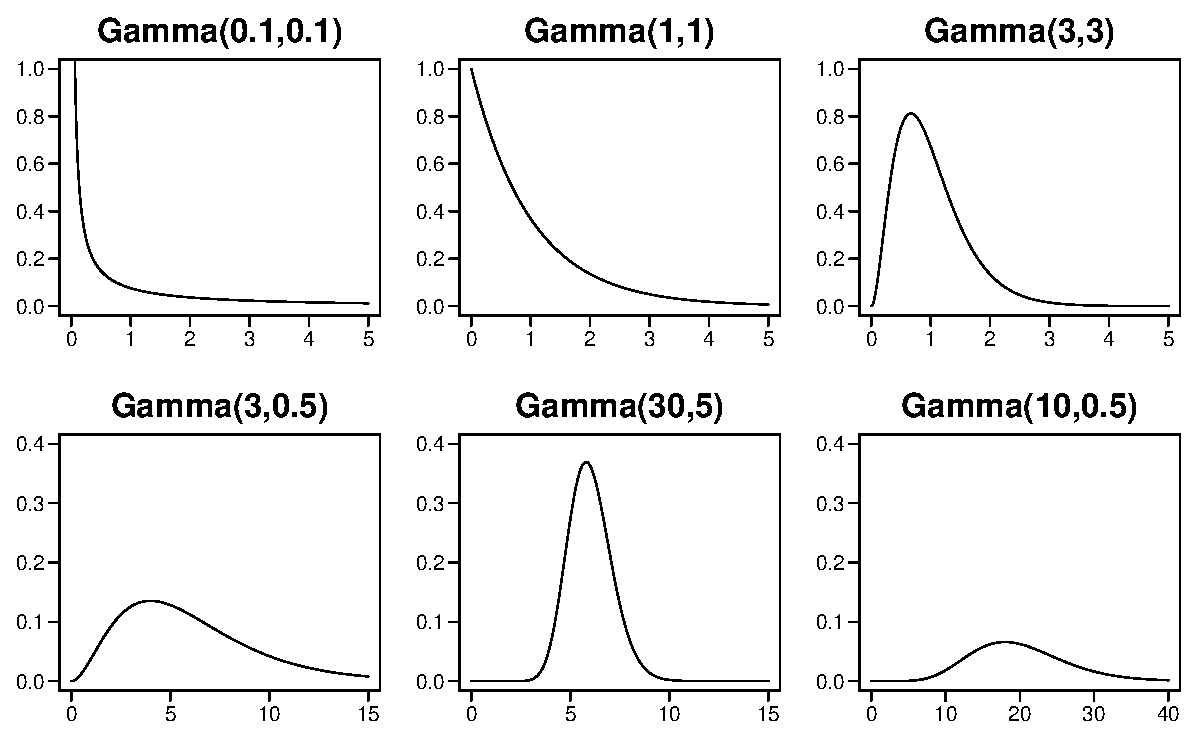
\includegraphics{Figures/gammas.pdf}}
\end{frame}

%%%%%%%%%%%%%%%%%%%%%%%%%%%%%%%%%%%%%%%%%%%%%%%%%%%%%%%%%%%%%%%%%%%%%%%
\frame{\frametitle{Combining likelihood and prior}
This implies the following posterior
\alert{\begin{eqnarray*}
p(\mu \mid \mathbf{y}) &\propto& p(\mu)\,p(\mathbf{y} \mid \mu) \\[3pt]
  &=& \frac{b^a}{\Gamma(a)}\mu^{a-1}e^{-b\mu}\prod_{i=1}^n e^{-\mu}\frac{\mu^{y_i}}{y_i !} \\[3pt]
  & \propto & \mu^{a+n\overline{y}-1} e^{-(b+n)\mu}\\[3pt]
 & = & \mathrm{Gamma}(a + n\overline{y} ,\, b + n)
\end{eqnarray*}
}
The posterior is another (different) Gamma distribution
\begin{equation*} \vspace{-0.1cm}
E(\mu \mid \mathbf{y})= \frac{a + n\overline{y} }{ b + n} = \overline{y}\left(\frac{n}{n +b}
\right) + \frac{a}{b}\left(1-\frac{n}{n + b}\right)
\end{equation*}

So posterior mean is a compromise between the prior mean $\frac{a}{b}$ and the sample mean ($\overline{y}$)
}
%%%%%%%%%%%%%%%%%%%%%%%%%%%%%%%%%%%%%%%%%%%%%%%%%%%%%%%%%%%%%%%%%%%%%%%%

\frame{
\frametitle{Example: Estimation of disease risk in a single area}

Often interested in estimating the \alert{rate} or \alert{relative risk}
rather than the \alert{mean} for Poisson data:

\begin{itemize}
\item Suppose we observe $y=5$ cases of leukaemia in one region,
   with age-sex-standardised expected number of cases $E$ = 2.8\vspace{0.5mm}
 \item Assume Poisson likelihood for $y$ with mean $\mu = \lambda \times
E$,
   where $\lambda$ is the unknown relative risk:
   $$p(y \mid  \lambda, E) = \frac{(\lambda E)^{y}e^{-\lambda E} }{y!}$$\vspace{-2mm}
 \item Assume Gamma($a$, $b$) prior for the relative risk $\lambda$:
   $$p(\lambda)  =  \frac{b^a}{\Gamma(a)} \lambda^{a-1} e^{-b \lambda} $$\vspace{-3mm}
 \item Posterior for $\lambda$ is then
\alert{ \begin{eqnarray*}
   p(\lambda \mid  y, E) &\propto & \frac{b^a}{\Gamma(a)} \lambda^{a-1} e^{-b \lambda}
                        \frac{(\lambda E)^{y}e^{-\lambda E} }{y!}\\[2pt]
   &\propto& \lambda^{a+y-1} e^{-(b+E) \lambda} = \hbox{Gamma}(a+y, b+E)
   \end{eqnarray*}
   }
\end{itemize}
}

\frame{
\frametitle{Class exercise: Comparing priors}

\begin{enumerate}
\item Suppose we wish to express vague prior information about $\lambda$\vspace{1mm}
\begin{itemize}
  \item A Gamma(0.1, 0.1) distribution represents a prior for the relative
     risk $\lambda$\vspace{1mm}
    \item What are the prior mean and variance?\vspace{1mm}
    \item What are the parameters of the posterior distribution? What is the posterior mean?\vspace{2mm}
\end{itemize}


\item Alternatively, we may have strong prior information in the form of a $\hbox{Gamma(48,40)}$\vspace{1mm}
\begin{itemize}
    \item What are the prior mean and variance?\vspace{1mm}
    \item What are the parameters of the posterior distribution? What is the posterior mean?\vspace{2mm}
\end{itemize}
\end{enumerate}

Compare the two priors and the two posteriors. What can you conclude?
}




\frame{
\frametitle{Summary}

For all these examples, we see that \vspace{1mm}
\begin{itemize}
\item the posterior mean is a compromise between the prior mean and the sample mean\vspace{1mm}
\item the posterior standard deviation is less than each of the
      prior standard deviation and the standard error\vspace{2mm}
\end{itemize}
 \begin{quote}
{\it  `A Bayesian is one who, vaguely expecting  a horse and
catching a glimpse of a donkey, strongly concludes he has seen a
mule'}  (Senn, 1997)
\end{quote}

 As $n\rightarrow \infty$, \vspace{1mm}
 \begin{itemize}
 \item the posterior mean $\rightarrow$ the sample mean\vspace{1mm}
\item the posterior standard deviation $\rightarrow$ the standard error\vspace{1mm}
\item the posterior does not depend on the prior
\end{itemize}

}
%%%%%%%%%%%%%%%%%%%%%%%%%%%%%%%%%%%%%%%%%%%%%%%%%%%%%%%%%%%%%%%%%%%%%%%%

\frame{

\frametitle{Summary [continued]}

\begin{itemize}
\item When the posterior is in the same family as the prior then we have what is known as \alert{conjugacy}\vspace{1mm}
\item This has the advantage that prior parameters can usually be interpreted as a \alert{prior sample}\vspace{1mm}
\item Examples include:
\renewcommand{\arraystretch}{1.1}
\begin{center}
\begin{tabular}{cccc}
  Likelihood  & Parameter &  Prior   & Posterior \\ 
    Normal & mean & Normal  &Normal \\
  Normal & precision & Gamma  & Gamma \\
  Binomial & success prob. & Beta &  Beta  \\
  Poisson & rate or mean & Gamma & Gamma \\
\end{tabular}
\end{center}
\renewcommand{\arraystretch}{1}\vspace{1mm}
\item Conjugate prior distributions are mathematically convenient, but do not
   exist for all likelihoods, and can be restrictive \vspace{1mm}
\item Computations for non-conjugate priors are harder, but possible using MCMC (see Lecture 4)
\end{itemize}
}
